Understanding and predicting survey performance includes modeling the likely input telemetry, the expected performance of the telescope and observatory, as well as understanding the survey strategy and its interaction with science outcomes.

At this point in commissioning, the operations of the observatory are focused on obtaining specific observations, with very different strategies than will be employed during operations. This includes very different configurations of the Feature Based Scheduler. Thus, we are not fully testing the Feature Based Scheduler as it would be used in operations yet, and have few comments about issues that may be related specifically to survey strategy implementation. 

However, we can begin to evaluate how our models may be validated or not by the currently acquired observations. Since observations were acquired for many purposes, and sometimes purposefully in or out of focus, the science program BLOCK-320 provides very useful comparison points. In-focus images taken as part of AOS triplets can also be useful for some purposes. And BLOCK-T345 provided an example of slews that are similar to how a standard survey pattern may execute. 

As we are pulling information about zeropoints, sky background, and measured image psf from the ConsDb, we are using values populated by Rapid Anaysis, running on the summit. These values are only populated for ACQ or OBJECT images where existing calibration data is available. We also use the bad visit list maintained by DM (the \texttt{excluded\_visits} repo) to remove on the order of 100 visits which are clearly marked as bad -- typically due to trails. This leaves us with 5008 exposures from the ComCam commissioning period.

The throughput curves available in \texttt{syseng\_throughputs}, the repository that tracks current system engineering summaries of full-focal-plane throughputs, can be used to predict zeropoints for average ITL CCDs. See \url{https://github.com/lsst-pst/syseng\_throughputs/blob/main/notebooks/InterpolateZeropoint.ipynb}, where a simple interpolation function for filter and airmass is defined for the current throughputs (v1.9).  Looking at only the science program visits (BLOCK-320 and PP-SURVEY), where images could be expected to be in the best possible focus and obtained under more controlled sky conditions (and where all images have 30 second exposures), we can compare the predicted 30s zeropoints to the reported median visit zeropoints in the ConsDB (the column \texttt{visit1\_quicklook.zero\_point\_median}), as shown in \figRef{zeropoints}. It is worth noting that the $u$ band is a significant outlier in this comparison of predicted versus measured zeropoint; we believe this is the same issue as discussed in \secRef{absolutethroughputs}, so is the result of either a miscalibration in the synthetically-derived reference catalog generated for zeropoint calibration or a true underestimate of the system performance in $u$ band.  We find that the estimated zeropoints are fairly close to the achieved zeropoints, except in u band. The median offsets for the photometric nights in the science survey visits are:  u = -0.26, g = 0.14, r = 0.09, i = 0.10, z = 0.13, y = 0.18. 

We applied these offsets as corrections to the zeropoints for all visits, and after also adjusting the measured zeropoints for the exposure time, can compared 1 second predicted and adjusted zeropoints for all visits, as in \figRef{all_zeropoints}.  As an example of a non-photometric night, see also the visits from dayObs 20241210 shown in \figRef{zeropoints_dayobs_20241210}. 

\begin{figure}
    \centering
    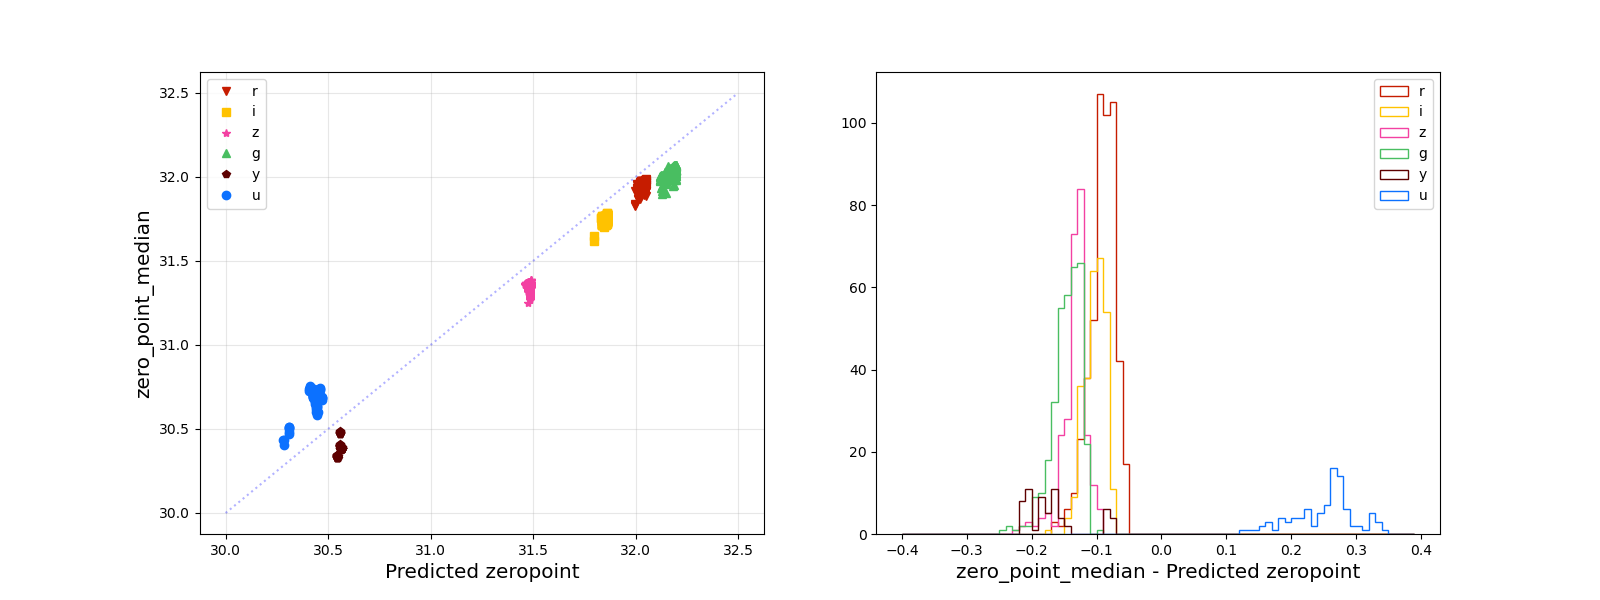
\includegraphics[width=0.7\textwidth]{sp/zeropoints.png}
    \caption{Predicted zeropoints from syseng\_throughputs (accounting for airmass) compared to measured zeropoints from \texttt{cdb\_lsst.comcam.visits1\_quicklook},  for BLOCK-320 and PP-SURVEy visits, excluding dayObs 20241210 which was highly non-photometric. The offsets between predicted and measured zeropoints seen here can be used as a quick approximation for an updated zeropoint and applied to all visits.}
    \label{fig:zeropoints}
    \end{figure}

\begin{figure}
    \centering
    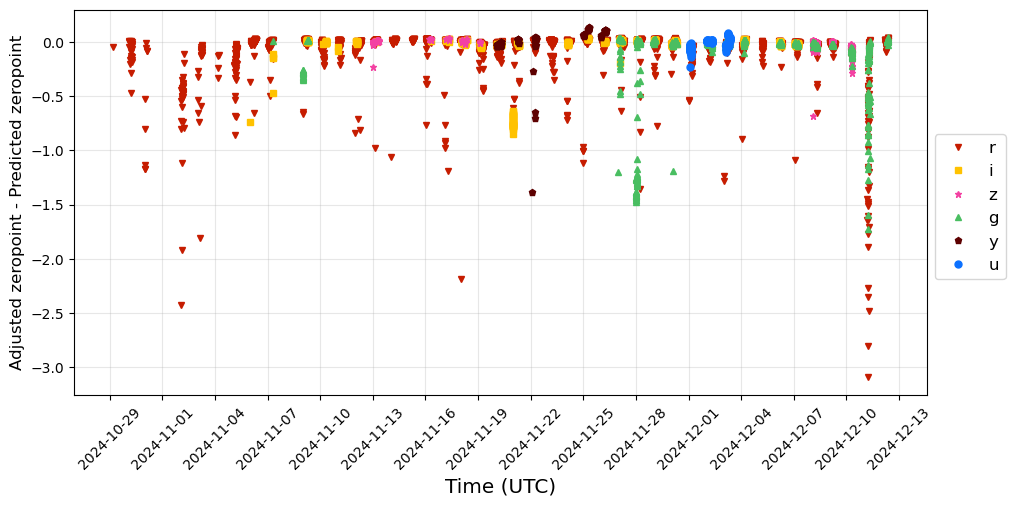
\includegraphics[width=0.7\textwidth]{sp/all_zeropoints.png}
    \caption{Measured zeropoints from \texttt{cdb\_lsst.comcam.visits1\_quicklook} adjusted for exposure time (\texttt{cdb\_lsst.comcam.visits1.shut\_time}) and our zeropoint offset, minus the predicted 1 second zeropoints from syseng\_throughputs (accounting for airmass), for all visits where the zeropoint information was reported. The offsets here are generally more indicative of transparency variations, but could also indicate other potential issues such as excessively out of focus images - many of the bad images on DM's list of excluded images were also identifiable as zeropoint outliers.}
    \label{fig:all_zeropoints}
    \end{figure}


\begin{figure}
    \centering
    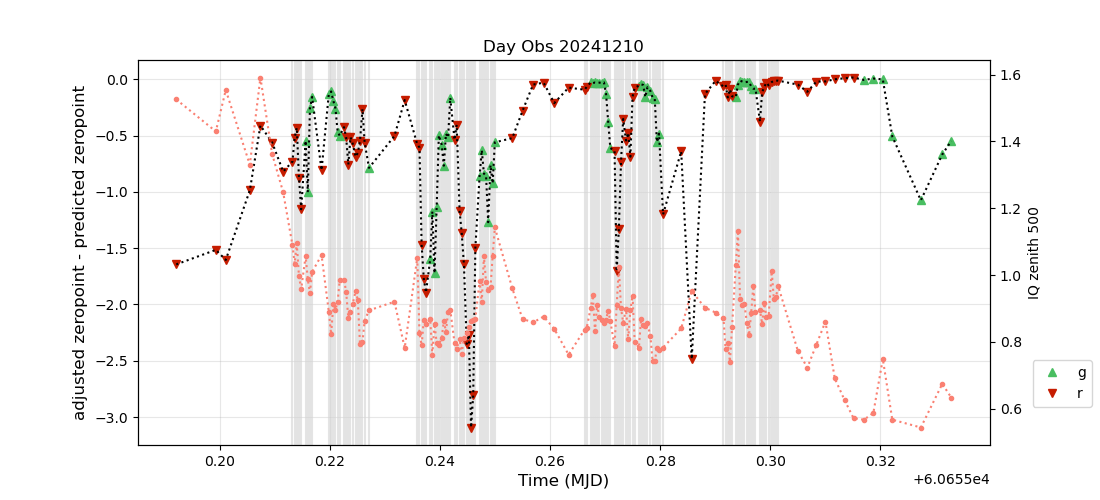
\includegraphics[width=0.7\textwidth]{sp/zeropoints_dayobs_20241210.png}
    \caption{Measured zeropoints from \texttt{cdb\_lsst.comcam.visits1\_quicklook} adjusted for exposure time (\texttt{cdb\_lsst.comcam.visits1.shut\_time}) and our zeropoint offset, minus the predicted 1 second zeropoints from syseng\_throughputs (accounting for airmass), for all ACQ and OBJECT visits on dayObs 20241210. The green upward triangles represent $g$ band while the red downward traingles represent $r$ band. The salmon dots indicate an extrapolated atmospheric seeing component, based on the \texttt{cdb\_lsst.comcam.visits1\_quicklook.psf\_sigma\_median} values adjusted to atmospheric seeing contribution at zenith, 500 nm. The gray lines indicate when a BLOCK-320 (science) visit was taking place. }
    \label{fig:zeropoints_dayobs_20241210}
    \end{figure}


Likewise, the survey simulations use a skybackground model as part of the model to determine five sigma visit depths and to choose observation pointings. The outputs available in the ConsDb include a \texttt{sky\_bg\_median} value, which is in counts per pixel. Together with an estimate of the platescale (0.2"/pixel) and a zeropoint, we can convert this into magnitudes per square arcsecond, to compare to the predicted values from the rubin\_scheduler skybrightness model. The results are shown in \figRef{sky}.  The values are also remarkably consistent, with a scatter of less than 0.15 magnitudes in all bands, and offsets within 0.1 magnitude except in y band, where the measured sky is 0.5 magnitudes brighter than expected. This is  within our expected errors in the skybackground model, particularly in y band where the sky is quite variable and harder to model.

\begin{figure}
    \centering
    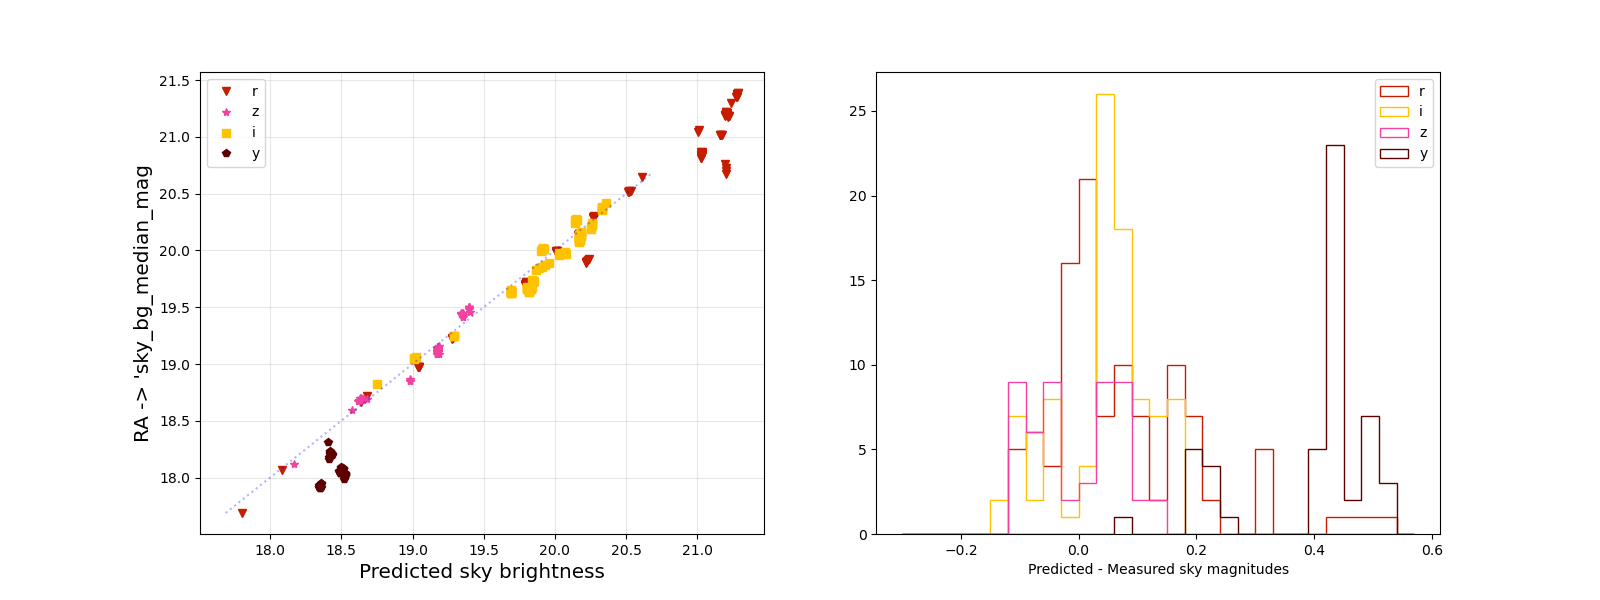
\includegraphics[width=0.8\textwidth]{sp/sky.png}
    \caption{Predicted skybrightness values from \texttt{rubin\_sim.skybrightness} compared to
      \texttt{sky\_bg\_median} converted to mags per sq arcsecond  from  from \texttt{visits1\_quicklook}.}
    \label{fig:sky}
    \end{figure}


We look forward to comparing seeing performance to survey predictions. Initial estimates indicate that the mean seeing for these visits was around 1.12 arcseconds, which isn't out of line with longer term survey expectations, especially given that we remain in the early stages of commissioning.

\begin{figure}
    \centering
    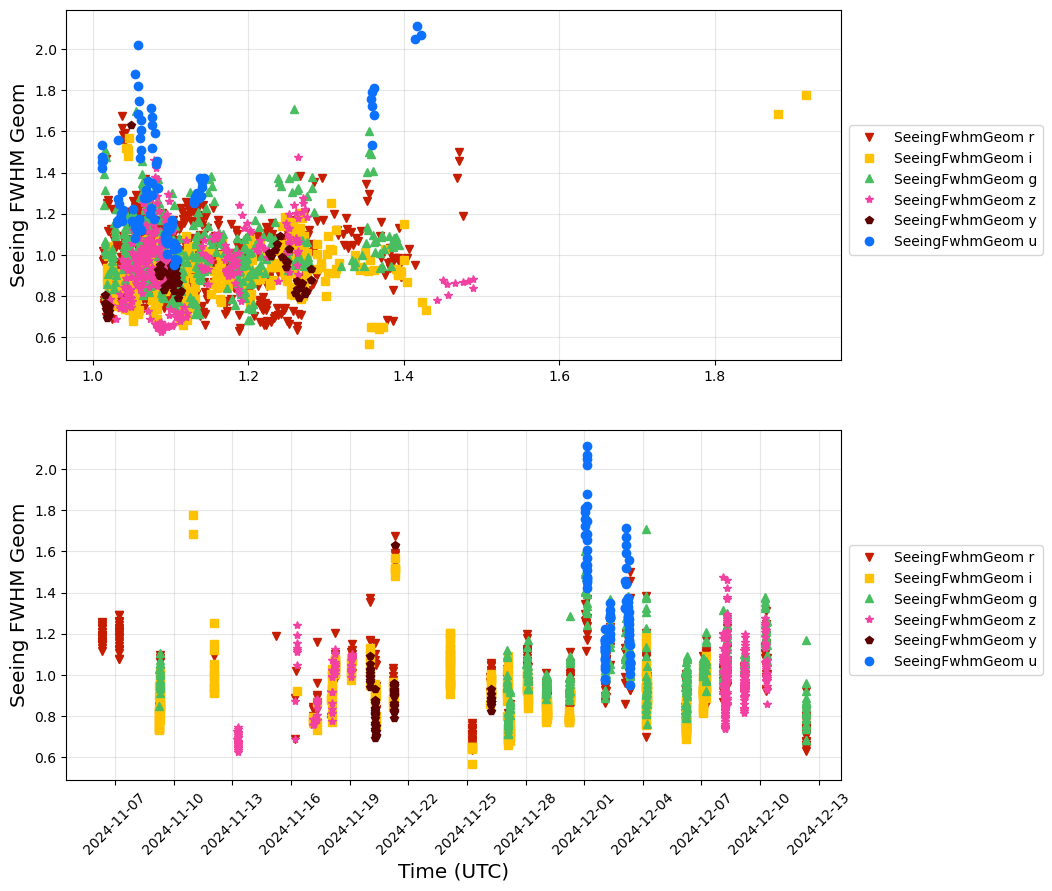
\includegraphics[width=0.8\textwidth]{sp/seeing.png}
    \caption{Converting \texttt{psf\_sigma\_median} into the single-gaussian effective seeing PSF values.}
    \label{fig:seeing}
    \end{figure}


Remaining questions include the efficiency of observations, and in particular the likelihood of whether a single snap will be sufficient.

\begin{figure}
    \centering
    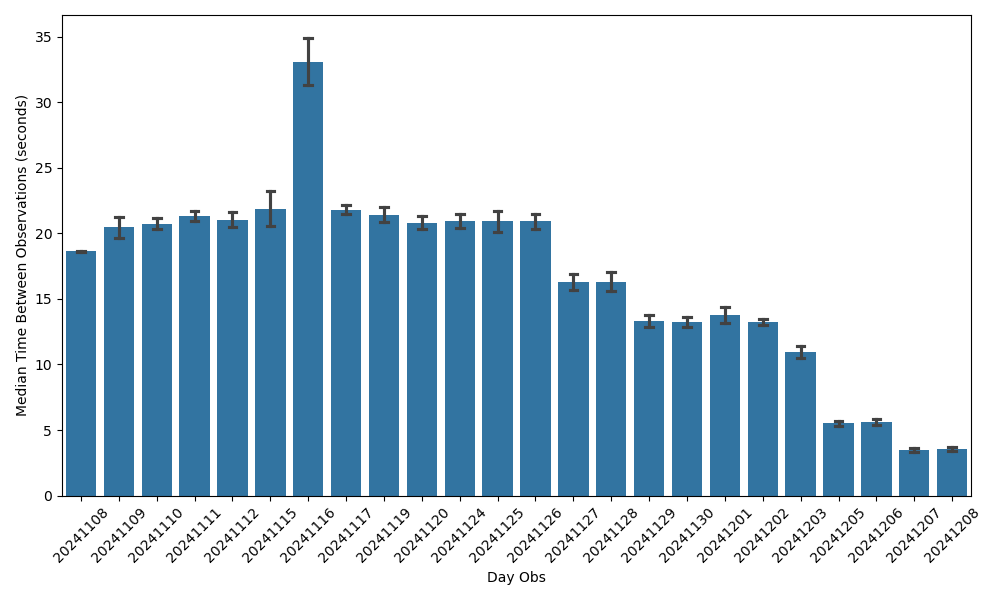
\includegraphics[width=0.7\textwidth]{sp/timeBetweenExposures20241208.png}
    \caption{Time between successive visits for Science Pipelines commissioning observations.}
    \label{fig:time_between_visits}
\end{figure}